\documentclass[prb,12pt]{revtex4-2}

\usepackage{amsmath, amssymb,physics,amsfonts,amsthm}
\usepackage{enumitem}
\usepackage[most]{tcolorbox}
\usepackage{cancel}
\usepackage{booktabs}
\usepackage{tikz}
\usepackage{hyperref}
\usepackage{enumitem}
\usepackage{transparent}
\usepackage{float}
\usepackage{multirow}
\usepackage{subcaption}
\newtheorem{Theorem}{Theorem}
\newtheorem{Proposition}{Theorem}
\newtheorem{Lemma}[Theorem]{Lemma}
\newtheorem{Corollary}[Theorem]{Corollary}
\newtheorem{Example}[Theorem]{Example}
\newtheorem{Remark}[Theorem]{Remark}
\theoremstyle{definition}
\newtheorem{Problem}{Problem}
\theoremstyle{definition}
\newtheorem{Definition}[Theorem]{Definition}
\newenvironment{parts}{\begin{enumerate}[label=(\alph*)]}{\end{enumerate}}
%tikz	
\tcbset{breakable=true,toprule at break = 0mm,bottomrule at break = 0mm}
\usetikzlibrary{patterns}
\usetikzlibrary{matrix}
\usepackage{pgfplots}
\pgfplotsset{compat=1.18}
% definitions of number sets
\newcommand{\N}{\mathbb{N}}
\newcommand{\R}{\mathbb{R}}
\newcommand{\Z}{\mathbb{Z}}
\newcommand{\Q}{\mathbb{Q}}
\newcommand{\C}{\mathbb{C}}
\allowdisplaybreaks
\begin{document}
\title{Gewöhnliche Differentialgleichungen Hausaufgaben Blatt 2}
	\author{Jun Wei Tan}
	\email{jun-wei.tan@stud-mail.uni-wuerzburg.de}
	\affiliation{Julius-Maximilians-Universit\"{a}t W\"{u}rzburg}
	\date{\today}
	\maketitle
%\paragraph{Aufgabe 1.1}
\begin{parts}
	\item 
		\begin{center}
			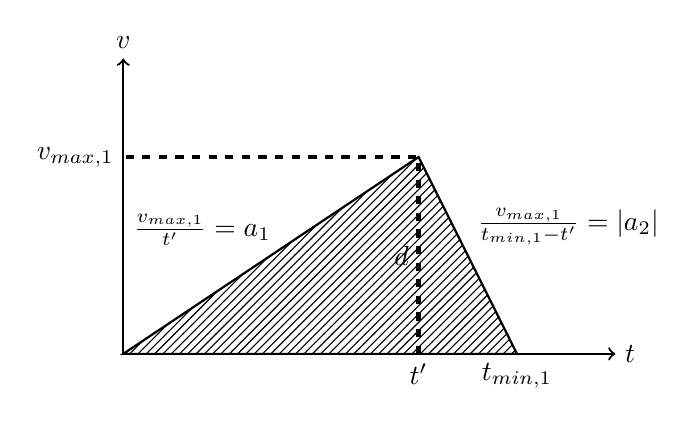
\begin{tikzpicture}[scale=2.5]
				\draw[thick, ->] (0,0) -- (2.5,0);
			\draw[thick, ->] (0,0) -- (0,1.5);
			\filldraw[thick, pattern = north east lines] (0,0) -- (1.5,1) -- (2,0) -- cycle;
			\draw (0,1.5) node[anchor=south] {$v$};
			\draw (2.5,0) node[anchor=west] {$t$};
			\draw (2,0) node[anchor=north] {$t_{min,1}$};
			\draw[ultra thick, dashed] (1.5,0) -- (1.5,1) -- (0,1);
			\draw (0,1) node[anchor=east] {$v_{max,1}$};
			\draw (1.5,0) node[anchor=north] {$t'$};
			\draw (0.4,0.5) node[anchor=south] {$\frac{v_{max,1}}{t'}=a_1$};
			\draw (1.75,0.5) node[anchor=south west] {$\frac{v_{max,1}}{t_{min,1}-t'} = |a_2|$};
			\draw (1.5,0.5) node[anchor=east] {$d$};
			\end{tikzpicture}
		\end{center}
		Man löst die Gleichungen
		\begin{align}
			\frac{1}{2}(v_{max,1})(t_{min,1})=&d\label{eqn1}\\
			v_{max,1}=&a_1t'\label{eqn2}\\
			v_{max,1}=&(t'-t_{min,1})a_2\label{eqn3}
		\end{align}
		Aus \eqref{eqn2} folgt $t'=v_{max,1} / a_1$. Wir setzen das in \eqref{eqn3} ein. Es ergibt sich
		\[
			v_{max,1}=\left( \frac{v_{max,1}}{a_1}-t_{min,1} \right) a_2
		.\] 
		Daraus folgt:
		\[
			v_{max,1}\left( 1-\frac{a_2}{a_1} \right) =-t_{min,1}a_2
		.\] 
	\item 	Noch einmal setzen wir das in \eqref{eqn1} ein:
		\[
			\frac{1}{2}\left[ -t_{min,1}a_2\left( 1-\frac{a_2}{a_1} \right)^{-1} \right] \left( t_{min,1} \right) =d 
		.\] 
		Die L\"{o}sung ist
		\[
			t_{min,1}=\boxed{\left[ -\frac{2d}{a_2}\left( 1-\frac{a_2}{a_1} \right)  \right]^{1 / 2}}
		.\] 
		Aus \eqref{eqn1} folgt
		\[
			v_{max,1}=\frac{2d}{t_{mn,1}}
		.\] 
		Also
		\[
			v_{max,1}=\boxed{\left[ -\frac{1-\frac{a_2}{a_1}}{2a_2d} \right]^{-1 / 2}} 
		.\] 
	\item 
		\begin{center}
			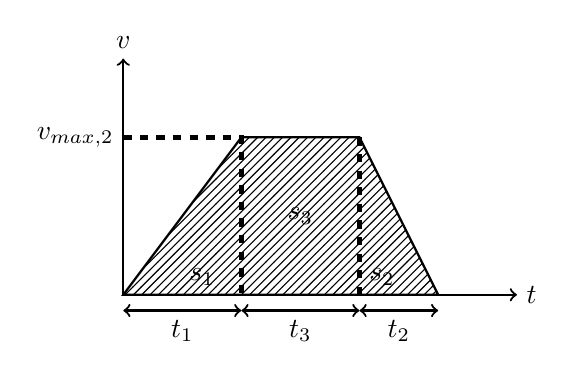
\begin{tikzpicture}[scale=2]
				\draw[thick, ->] (0,0) --(2.5,0);
				\draw[thick, ->] (0,0) -- (0,1.5);
				\filldraw[thick,pattern = north east lines] (0,0) -- (0.75,1) -- (1.5,1) -- (2,0) -- cycle;
				\draw[ultra thick, dashed] (0,1) -- (0.75,1) -- (0.75,0);
				\draw[ultra thick, dashed] (1.5,1) -- (1.5,0);
				\draw (0,1) node[anchor=east] {$v_{max,2}$};
				\draw[thick, <->] (0,-0.1) -- (0.75,-0.1);
				\draw (0.375,-0.1) node[anchor=north] {$t_1$};
				\draw (2.5,0) node[anchor=west] {$t$};
				\draw[thick,<->] (1.5,-0.1) -- (2,-0.1);
				\draw (1.75,-0.1) node[anchor=north] {$t_2$};
				\draw (0,1.5) node[anchor=south] {$v$};
				\draw (0.5,0) node[anchor=south] {$s_1$};
				\draw (1.5,0) node[anchor=south west] {$s_2$};
				\draw (1.125,0.5) node {$s_3$};
				\draw[thick,<->] (0.75,-0.1) -- (1.5,-0.1);
				\draw (1.125,-0.1) node[anchor=north] {$t_3$};
			\end{tikzpicture}
		\end{center}
		Es gilt
		\begin{align*}
			t_1=&\frac{v_{max,2}}{a_1}\\
			t_2=&-\frac{v_{max,2}}{a_2}\\
			s_1=&\frac{1}{2}a_1t_1^2=\frac{v_{max,2}^2}{2a_1}\\
			s_2=&\frac{1}{2}v_{max,2}t_2=-\frac{v_{max,2}^2}{2a_2}\\
			s_3=&v_{max,2}t_3=d-s_1-s_2\\
			t_3=&\frac{d-s_1-s_2}{v_{max,2}}\\
			=&\frac{d}{v_{max,2}}-\frac{v_{max,2}}{2a_1}+\frac{v_{max,2}}{2a_2}\\
			t_{min,2}=&t_1+t_2+t_3\\
			=&\frac{d}{v_{max,2}}+\frac{v_{max,2}}{2a_1}-\frac{v_{max,2}}{2a_2}\\
		\end{align*}

\end{parts}
\paragraph{Aufgabe 1.2}
\begin{center}
	\begin{tikzpicture}[scale=2.5]
		\draw[thick, ->] (0,0) -- (0,{(3-sqrt(3))/(1+sqrt(3))});
		\draw[thick, ->] (0,{(3-sqrt(3))/(1+sqrt(3))}) -- ++({0.4*cos(60)},{0.4*sin(60)});
		\draw (0,{(3-sqrt(3))/(2*(1+sqrt(3)))}) node[anchor=east] {$h_0$};
		\draw[thick, ->] (2,0) -- (2,1);\draw (2,0.5) node[anchor=west] {$h_1$};
		\draw[thick] (0,{(3-sqrt(3))/(1+sqrt(3))}) arc (150:60:{4/(1+sqrt(3))});
		\draw[thick,<->] (0,0) -- (2,0);
		\draw (1,0) node[anchor=north] {$l$};
	\end{tikzpicture}
\end{center}
\begin{gather*}
	x=v_0t\cos\theta\\
	y=v_0t\sin\theta-\frac{1}{2}gt^2\\
	y=x\tan\theta-\frac{gx^2}{2v_0^2\cos^2\theta}
\end{gather*}
Wir brauchen $y(l)=h_1-h_0$, oder
\[
h_1-h_0=l\tan\theta-\frac{gl^2}{2v_0^2\cos^2\theta}
.\] 
Daraus folgt
\[
v_0^2=\frac{gl^2}{2\cos^2\theta\left( l\tan\theta-(h_1-h_0) \right) }
.\] 

\begin{center}
	$l=h_1=1\text{ m},h_0=0\text{ m}$


	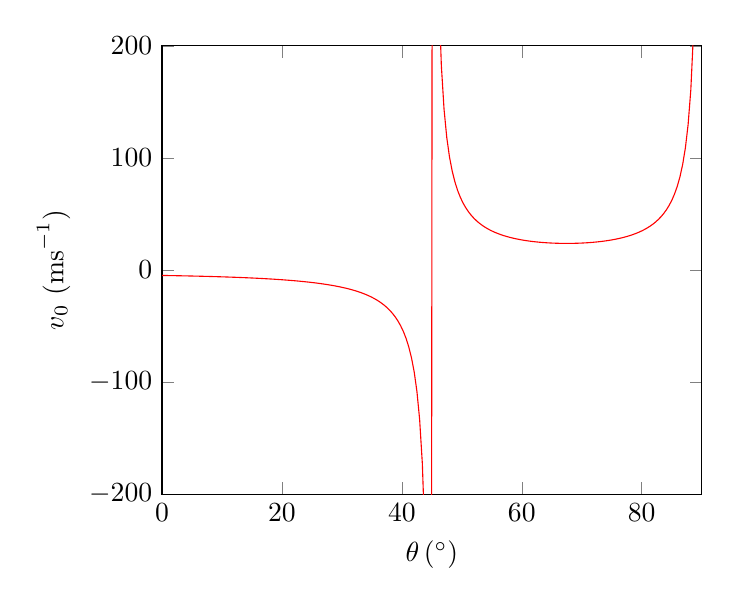
\begin{tikzpicture}
		\begin{axis}[ymin=-200,ymax=200,xmin=0,xmax=90,xlabel=$\theta\left( ^{\circ} \right) $,ylabel=$v_0\text{ (ms}^{-1})$]
\addplot[domain=0:90,color=red,samples=200]{9.81/(2*cos(x)*cos(x)*(tan(x)-1))};
\end{axis}
	\end{tikzpicture}
\end{center}
Es folgt daraus:
\[
y=x\tan\theta-(l\tan\theta-(h_1-h_0))\frac{x^2}{l^2}
.\] 
\paragraph{Aufgabe 1.3}
\begin{center}
	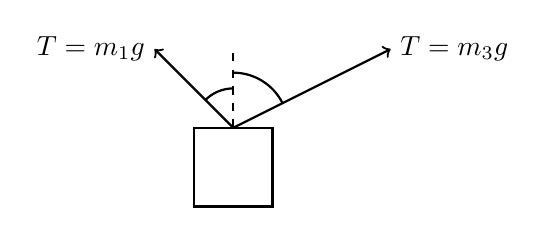
\begin{tikzpicture}
		\draw[thick] (-0.5,-1) rectangle (0.5,0);
		\draw[thick,->] (0,0) -- (-1,1);
		\draw[thick,->] (0,0) -- (2,1);
		\draw[thick, dashed] (0,0) -- (0,1);
		\draw[thick] (0,0.5) arc(90:135:0.5);
		\draw[thick] (0,0.7) arc(90:{atan(0.5)}:0.7);
		\draw (-1,1) node[anchor=east] {$T=m_1g$};
		\draw (2,1) node[anchor=west] {$T=m_3g$};
	\end{tikzpicture}
\end{center}
Es gilt
\begin{align*}
	x:& m_1g\sin\alpha=m_3g\sin\beta\\
	y:& m_1g\cos\alpha+m_3g\cos\beta=m_2g
\end{align*}
Also
\begin{align*}
	m_3=&m_1\frac{\sin\alpha}{\sin\beta}\\
	m_1\cos\alpha+m_1\frac{\sin\alpha}{\sin\beta}\cos\beta=&m_2\\
	m_1=&\frac{m_2}{\cos\alpha+\cos\beta\left( \frac{\sin\alpha}{\sin\beta} \right) }\\
	=& \frac{m_2\sin\beta}{\sin(\alpha+\beta)}\\
	m_3=&\frac{m_2\sin\alpha}{\sin(\alpha+\beta)}
\end{align*}
\begin{center}
	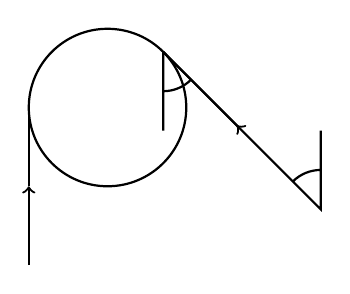
\begin{tikzpicture}
		\draw[thick] (0,0) circle (1);
		\draw[thick,->] (-1,-2) -- (-1,-1);
		\draw[thick] (-1,-1) -- (-1,0);
		\draw[thick,-<] ({1/sqrt(2)},{1/sqrt(2)}) -- ++(1,-1);
		\draw[thick] ({1/sqrt(2)},{1/sqrt(2)}) -- ++(2,-2) -- ++(0,1) -- ++(0,-0.5) arc(90:135:0.5);
		\draw[thick] ({1/sqrt(2)},{1/sqrt(2)}) -- ++(0,-1) -- ++(0,0.5) arc(-90:-45:0.5);
	\end{tikzpicture}
\end{center}
\begin{align*}
	\va F=&-\left[ \begin{pmatrix} 0 \\ -m_1g \end{pmatrix} +m_1g\begin{pmatrix} \sin\alpha \\-\cos\alpha  \end{pmatrix}  \right]\\
	=& m_1g\begin{pmatrix} -\sin\alpha \\ 1+\cos\alpha \end{pmatrix} 
\end{align*}
\paragraph{Aufgabe 1.4}
\begin{parts}
\item 
\noindent \\
	\begin{center}
		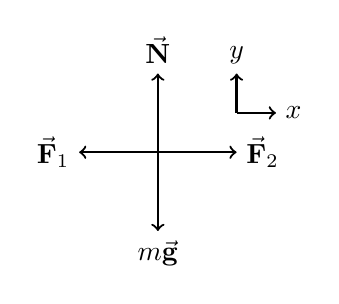
\begin{tikzpicture}
			\draw[thick,->] (0,0) -- (1,0);
			\draw (1,0) node[anchor=west] {$\va F_2$};
			\draw[thick, ->] (0,0) -- (-1,0);
			\draw (-1,0) node[anchor=east] {$\va F_1$};
			\draw[thick,->] (0,0) -- (0,1);
			\draw (0,1) node[anchor=south] {$\va N$};
			\draw (0,-1) node[anchor=north] {$m\va g$};
			\draw[thick, ->] (0,0) -- (0,-1);
			\draw[thick,->]	 (1,0.5) -- (1,1);
			\draw[thick, ->] (1,0.5) -- (1.5,0.5);
			\draw (1,1) node[anchor=south] {$y$};
			\draw (1.5,0.5) node[anchor=west] {$x$};
		\end{tikzpicture}
	\end{center}
\item $a_y=0$ (Zwangsbedingung), $a_x=\frac{1}{3m}\left(|F_2|-|F_1|\right)$
\item \noindent \\
	\begin{center}
		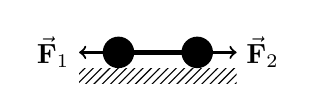
\begin{tikzpicture}[scale=1]
			\fill[pattern = north east lines] (0,-0.2) rectangle (2,0);
		\fill (0.5,0.2) circle (0.2);
	\fill (1.5,0.2) circle (0.2);
	\draw[thick, ->] (0.5,0.2) -- (0,0.2);
	\draw[thick, ->] (1.5,0.2) -- (2,0.2);
	\draw (0,0.2) node[anchor=east] {$\va F_1$};
	\draw (2,0.2) node[anchor=west] {$\va F_2$};
	\draw[ultra thick] (0.5,0.2) -- (1.5,0.2);
		\end{tikzpicture}
	\end{center}
	\[
	a_1=a_2=\frac{1}{3m}\left(|\va F_2|-|\va F_1| \right) 
	.\] 
\item \noindent \\
	\begin{center}
		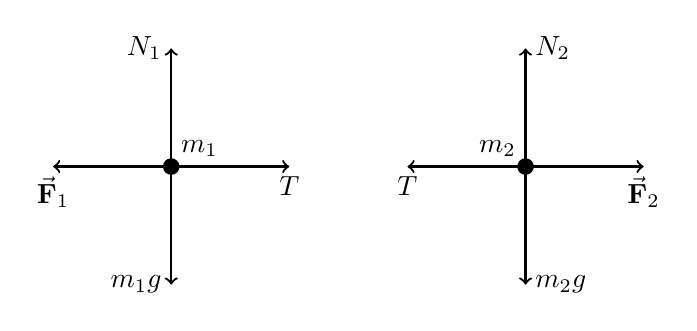
\begin{tikzpicture}[scale=1.5]
		\fill (0,0) circle (2pt);
		\draw[thick, ->] (0,0) -- (1,0);
		\draw[thick, ->] (0,0) -- (0,1);
		\draw[thick, ->] (0,0) -- (-1,0);
		\draw[thick, ->] (0,0) -- (0,-1);
	\fill (3,0) circle (2pt);
	\draw[thick, ->] (3,0) -- (4,0);
	\draw[thick, ->] (3,0) -- (3,1);
	\draw[thick, ->] (3,0) -- (3,-1); 
	\draw[thick, ->] (3,0) -- (2,0);
	\draw (1,0) node[anchor=north] {$T$};
	\draw (0,1) node[anchor=east] {$N_1$};
	\draw (0,-1) node[anchor=east] {$m_1g$};
	\draw (-1,0) node[anchor=north] {$\va F_1$};
	\draw (4,0) node[anchor=north] {$\va F_2$};
	\draw (2,0) node[anchor=north] {$T$};
	\draw (3,1) node[anchor=west] {$N_2$};
	\draw (3,-1) node[anchor=west] {$m_2g$};
	\draw (0,0) node[anchor=south west] {$m_1$};
	\draw (3,0) node[anchor=south east] {$m_2$};
		\end{tikzpicture}
	\end{center}
\item 
	\begin{align*}
		m_1a=&T-F_1\\
		m_2a=& F_2-T\\
		(m_1+m_2)a=&T-F_1+F_2-T\\
		=&F_2-F_1\\
		=&3ma\\
		a=&\frac{1}{3m}\left( F_2-F_1 \right) 
	\end{align*}
\end{parts}

%	\begin{Problem}
	Es seien die Punkte $x_0, x_1, \dots, x_n$ mit $x_i \in \R$ gegeben. Wir definieren den Operator
	\[
		\Phi:\R_{\le n}[x]\to \R^{n+1}, p\to y, \text{ mit }p(x_i)=y_i, i=0,\dots,n
	\] 
	wobei wir mit $\R_{\le n}[x]$ den Raum der Polynome mit reellen Koeffizienten vom Grad höchsten $n$ bezeichnen und $p(x)$ die Auswertung des Polynoms $p$ im Punkt $x$ beschreibt.
	\begin{parts}
		\item  Zeigen Sie: Sind die Punkte $x_i$ paarweise verschieden, so ist die Abbildung $\Phi$ wohldefiniert und isomorph. (Eine Konsequenz hieraus ist die eindeutige Lösbarkeit der Polynominterpolation.)
		\item Was passiert, wenn Sie nicht fordern, dass die $x_i$ paarweise verschieden sind? Kann $\Phi$ im Allgemeinen noch injektiv (surjektiv) sein?
	\end{parts}
\end{Problem}
\begin{proof}
	\begin{parts}
\item Injektiv: Nehme an, dass es zwei unterschiedliche Polynome $p_1$, $p_2$ gibt, mit $p_1(x_i)=p_2(x_i)\forall i=0,\dots,n$. Dann ist $p(x):=p_1(x)-p_2(x)$ auch ein Polynom, mit $p(x_i):=0\forall i\in \{0,\dots,n\}$. Weil  $ \deg(p)\le n$ist, folgt daraus, dass $\forall x,p(x)=0, p_1(x)=p_2(x)$. Das ist ein Widerspruch.

	Surjektive: Sei $(y_0,\dots,y_n)\in \R^{n+1}$. Dann ist
	\[
	p(x)=(x-y_0)(x-y_1)\dots(x-y_n)
	\]
	auch ein Polynom mit $\Phi(p)=(y_0,\dots,y_n)$.

	Linearität: Sei $p_1(x),p_2(x)\in \R_{\le n}[x], a\in \R$. Sei auch $p(x)=p_1(x)+p_2(x)$. Es gilt dann
	\[
	p(x_i)=p_1(x_i)+p_2(x_i),i=0,\dots,n\] und daher
	\[
	\Phi(p)=\Phi(p_1+p_2)=\Phi(p_1)+\Phi(p_2)
	.\] 
	Es gilt auch, f\"{u}r $p(x):=ap_1(x)$, dass
	\[
	p(x_i)=ap_1(x_i), i=0,\dots,n
	,\]
	und daher
	\[
	\Phi(p)=\Phi(ap_1)=a\Phi(p_1)
	.\] 
\item Nein. Sei, zum Beispiel, $n=1$, $x_0=x_1=0$. Dann gilt
	\begin{align*}
		\Phi(x)=&(0,0)^T\\
		\Phi(x^2)=&(0,0)^T
	\end{align*}
	Aber die zwei Polynome sind ungleich.
	\end{parts}
\end{proof}

\begin{Problem}
	\begin{parts}	
	\item Es sei eine Matrix $A \in \mathbb{K}^{n\times n}$ gegeben. Wir bilden die erweiterte Matrix
	\[
		B=(A|1_n)\]
		mit $1_n$ die Einheitsmatrix in $\R^n$. Zeigen Sie: $A$ ist genau dann invertierbar, wenn $A$ durch elementare Zeilenumformung in die Einheitsmatrix überführt werden kann. Verfizieren Sie weiterhin: Werden die dafür benötigten Zeilenumformungen auf ganz $B$ angewendet, so ergibt sich im hinteren Teil, wo zu Beginn die Einheitsmatrix stand, genau $A^{-1}$.
	\item Es sei nun
		\[
			A=\begin{pmatrix} 1 & 0 & 0 & 1\\0 & -1 & 2 & 0 \\ 0 & 0 & 0 & -2\\3 & 0 & 1 & 2 \end{pmatrix} 
		.\] 
		Bestimmen Sie $A^{-1}$.
	\end{parts}
\end{Problem}
\begin{proof}
	\begin{parts}
	\item Definiert $(x,y),x\in \mathbb{K}^n,y\in\mathbb{K}^m$ durch $\mathbb{K}^{n+m}\ni(x,y)=(x_1,\dots,x_n,y_1,\dots,y_n)$. Eine solche erweiterte Matrix bedeutet eine Gleichungssystem durch
		\[
		B(x, -y)=Ax-1_ny=0
		,\]
		wobei $x,y\in \mathbb{K}^n$. F\"{u}r jeder $x\in\mathbb{K}^n$ gibt es $y\in \mathbb{K}^n,$ so dass $B(x,-y)=0$. Nehme an, dass wir durch elementare Zeilenumformung
		\[
		B=(A|1_n)\to (1_n, A'):=B'
		\]
		kann. Die Gleichungssystem ist dann $x=A'y$. Dadurch können wir f\"{u}r jeder  $y\in\mathbb{K}^n$ eine $A'y=x\in\mathbb{K}^n$ rechnen, f\"{u}r die gilt, dass $Ax=y$. Das heißt, dass $A'=A^{-1}$. 
	\item
		{\allowdisplaybreaks
		\begin{gather*}
			\left(
\begin{array}{cccc|cccc}
 1 & 0 & 0 & 1 & 1 & 0 & 0 & 0 \\
 0 & -1 & 2 & 0 & 0 & 1 & 0 & 0 \\
 0 & 0 & 0 & -2 & 0 & 0 & 1 & 0 \\
 3 & 0 & 1 & 2 & 0 & 0 & 0 & 1 \\
\end{array}
\right) \xrightarrow{R_4-3R_1} \left(
\begin{array}{cccc|cccc}
 1 & 0 & 0 & 1 & 1 & 0 & 0 & 0 \\
 0 & -1 & 2 & 0 & 0 & 1 & 0 & 0 \\
 0 & 0 & 0 & -2 & 0 & 0 & 1 & 0 \\
 0 & 0 & 1 & -1 & -3 & 0 & 0 & 1 \\
\end{array}
\right) \xrightarrow{R_2\times -1}\\ \left(
\begin{array}{cccc|cccc}
 1 & 0 & 0 & 1 & 1 & 0 & 0 & 0 \\
 0 & 1 & -2 & 0 & 0 & -1 & 0 & 0 \\
 0 & 0 & 0 & -2 & 0 & 0 & 1 & 0 \\
 0 & 0 & 1 & -1 & -3 & 0 & 0 & 1 \\
\end{array}
\right) \xrightarrow{R_3\leftrightarrow R_4} \left(
\begin{array}{cccc|cccc}
 1 & 0 & 0 & 1 & 1 & 0 & 0 & 0 \\
 0 & 1 & -2 & 0 & 0 & -1 & 0 & 0 \\
 0 & 0 & 1 & -1 & -3 & 0 & 0 & 1 \\
 0 & 0 & 0 & -2 & 0 & 0 & 1 & 0 \\
\end{array}
\right) \xrightarrow{R_2+2R_3}\\ \left(
\begin{array}{cccc|cccc}
 1 & 0 & 0 & 1 & 1 & 0 & 0 & 0 \\
 0 & 1 & 0 & -2 & -6 & -1 & 0 & 2 \\
 0 & 0 & 1 & -1 & -3 & 0 & 0 & 1 \\
 0 & 0 & 0 & -2 & 0 & 0 & 1 & 0 \\
\end{array}
\right) \xrightarrow{R_2-R_4} \left(
\begin{array}{cccc|cccc}
 1 & 0 & 0 & 1 & 1 & 0 & 0 & 0 \\
 0 & 1 & 0 & 0 & -6 & -1 & -1 & 2 \\
 0 & 0 & 1 & -1 & -3 & 0 & 0 & 1 \\
 0 & 0 & 0 & -2 & 0 & 0 & 1 & 0 \\
\end{array}
\right) \xrightarrow{R_4\times -\frac{1}{2}}\\ \left(
\begin{array}{cccc|cccc}
 1 & 0 & 0 & 1 & 1 & 0 & 0 & 0 \\
 0 & 1 & 0 & 0 & -6 & -1 & -1 & 2 \\
 0 & 0 & 1 & -1 & -3 & 0 & 0 & 1 \\
 0 & 0 & 0 & 1 & 0 & 0 & -\frac{1}{2} & 0 \\
\end{array}
\right) \xrightarrow{R_1-R_4} \left(
\begin{array}{cccc|cccc}
 1 & 0 & 0 & 0 & 1 & 0 & \frac{1}{2} & 0 \\
 0 & 1 & 0 & 0 & -6 & -1 & -1 & 2 \\
 0 & 0 & 1 & -1 & -3 & 0 & 0 & 1 \\
 0 & 0 & 0 & 1 & 0 & 0 & -\frac{1}{2} & 0 \\
\end{array}
\right) \xrightarrow{R_3+R_4} \\\left(
\begin{array}{cccc|cccc}
 1 & 0 & 0 & 0 & 1 & 0 & \frac{1}{2} & 0 \\
 0 & 1 & 0 & 0 & -6 & -1 & -1 & 2 \\
 0 & 0 & 1 & 0 & -3 & 0 & -\frac{1}{2} & 1 \\
 0 & 0 & 0 & 1 & 0 & 0 & -\frac{1}{2} & 0 \\
\end{array}
\right)
		\end{gather*}
	}
	\end{parts}
\end{proof}
\begin{Problem}
	Es seien die Vektorräume $V, W$ über $\mathbb{K}$ gegeben mit $\dim(V) = n$ und $\dim(W ) = m$. Wir betrachten eine lineare Abbildung
	\[
	T:V\to W, v\to T(v)\] 
Seien $B_V$ und $B_W$ Basen von $V$, bzw. $W$. Wir nehmen an $T$ ist nicht die konstante Nullabbildung. Beweisen Sie:
\begin{parts}
\item Der Kern von $_{B_W}[T]_{B_V}$ ist entweder trivial (d.h. nur die 0) oder hängt nur von der Wahl von $B_V$ ab, aber nicht von $B_W$.
\item Das Bild von $_{B_W}[T]_{B_V}$ ist entweder der ganze $\mathbb{K}^m$ oder hängt nur von der Wahl von $B_W$ ab, aber nicht von $B_v$. 
\item Der Rang von $_{B_W}[T]_{B_V}$ ist unabh\"{a}ngig von $B_w$ und $B_V$.
aber nicht von $B_W$.
\end{parts}
\end{Problem}
\begin{proof}
Nach Korollar 5.43 gilt, f\"{u}r $A,A' \subseteq V$ und $B,B'\subseteq W$ Basen der Vektorräume $V$ und $W$ über $\mathbb{K}$, und $\Phi\in \text{Hom}(V,W)$.
 \[
	 _{B'}\left[ \Phi \right]_{A'}={}_{B'}[\text{id}_W]_B\cdot{}_B[\Phi]_A\cdot{}_A[\text{id}_V]_{A'}
.\] 
\begin{Lemma}
	Jeder Basiswechsel f\"{u}r sowohl $B_V$ als auch $B_W$ kann als zwei Basiswechseln interpretiert werden, wobei eine Basiswechsel nur $B_V$ verändert, und die andere nur $B_W$.
\end{Lemma}
\begin{proof}
	\[
		_{B'}\left[ \Phi \right]_{A'}={}_{B'}[\text{id}_W]_B\cdot{}_B[\Phi]_A\cdot{}_A[\text{id}_V]_{A'}={}_{B'}[\text{id}_W]_B\left( {}_B[\text{id}_W]_B\cdot {}_B[\Phi]_A\cdot {}_A[\text{id}]_{A'} \right) {}_A[\text{id}_V]_A
	.\]
	(In den Klammern gibt es zuerst ein Basiswechsel in $V$, dann ein Basiswechsel in $W$ ). Ein ähnliche Argument zeigt, dass wir zuerst ein Basiswechseln in $W$ betrachten kann.
\end{proof}
\begin{Corollary}
	In jedem Teilaufgabe muss man nur das Fall betrachten, in dem entweder $B_V$ oder $B_W$ sich verändert. 
\end{Corollary}
	\begin{parts}
	\item 
	\end{parts}
\end{proof}

	\begin{Problem}
	\begin{parts}
		\item  Berechnen Sie alle möglichen Matrixprodukte der folgenden Matrizen. Was muss jeweils für die Dimensionen erfüllt sein?
	 \begin{gather*}
		 A=\begin{pmatrix} 1 & -1 & 2 \\ 0 & 3 & 5 \\ 1 & 8 & 7 \end{pmatrix}, B=\begin{pmatrix} -1 & 0 & 1 & 0 \\ 0 & 1 & 0 & -1 \\ 1 & 0 & -1 & 0 \end{pmatrix} ,C=\begin{pmatrix} 1 \\ 0 \\ 8 \\ -7 \end{pmatrix}\\
		 D=\begin{pmatrix} -1 & 2 & 0 & 8 \end{pmatrix}, E=\begin{pmatrix} 1 & 4 \\ 0 & 5 \\ 6 & 8 \end{pmatrix} , F=\begin{pmatrix} -1 & 2 & 0 \end{pmatrix} .
	 \end{gather*}
 \item Eine Blockmatrix ist eine Matrix von der Form
	 \[
		 A=\begin{pmatrix} A_1 & A_3 \\ A_2 & A_4 \end{pmatrix} \] 
		 mit Matrizen $A_1\in \mathbb{K}^{n \times m}, A_2\in \mathbb{K}^{n'\times m}, A_3\in \mathbb{K}^{n \times m'}, A_4\in\mathbb{K}^{n'\times m'}$. Sei weiterhin
		 \[
			 B=\begin{pmatrix} B_1 & B_3 \\ B_2 & B_4 \end{pmatrix} \] 
			 mit ebenso Einträgen aus $\mathbb{K}$. Wer nun meint, die Multiplikation von A und B sei so simpel wie
			 \[
				 A\cdot B=\begin{pmatrix} A_1B_1+A_3B_2 & A_1B_3+A_3B_4 \\ A_2B_1+A_4B_2 & A_2B_3+A_4B_4 \end{pmatrix} \] 
hat tatsächlich recht. Beweisen Sie diese Formel und geben Sie gleichzeitig die $B_i'$s für die benötigten Matrizenräume an, sodass die Rechnung wohldefiniert ist.
 \end{parts}
\end{Problem}
\begin{proof}
	\begin{parts}
	\item F\"{u}r $A$ eine $n\times m$ Matrize, und $B$ eine $p\times q$ Matrize, ist $AB$ wohldefiniert, nur wenn $m=p$

		Die Matrizprodukte sind
		\begin{gather*}
			AB=\begin{pmatrix} 1 & -1 & -1 & 1\\5 & 3 & -5 & -3 \\ 6 & 8 & -6 & -8 \end{pmatrix}\\
			AE=\begin{pmatrix} 13 & 15 \\ 30 & 55 \\ 43 & 100 \end{pmatrix} \\
			FA=\begin{pmatrix} -1 & 7 & 8 \end{pmatrix}\\ 
			BC=\begin{pmatrix} 7 \\ -7 \\ -7 \end{pmatrix}\\
			CD=\begin{pmatrix} -1 & 2 & 0 & 8 \\ 0 & 0 & 0 & 0\\-8 & 16 & 0 & 64\\-7 & 14 & 0 & 56 \end{pmatrix}\\
			DC=(55)\\
			CF=\begin{pmatrix} -1 & 2 & 0 \\ 0 & 0 & 0 \\ -8 & 16 & 0\\-7 & 14 & 0 \end{pmatrix}\\ 
			FE=\begin{pmatrix} -1 & 6 \end{pmatrix} 
		\end{gather*}
	\item Wir brauchen $B_1\in\mathbb{K}^{m\times p},B_2\in\mathbb{K}^{m'\times p}, B_3\in\mathbb{K}^{m\times q}, B_4\in\mathbb{K}^{m'\times q}$ f\"{u}r $p,q\in \N$. Wir bezeichnen, f\"{u}r $v_1\in\mathbb{K}^a,v_2\in\mathbb{K}^b$, das Vektor $(v_1,v_2)\in\mathbb{K}^{a+b}$. Sei jetzt $v_1\in \mathbb{K}^p,v_2\in\mathbb{K}^q$.
		{\allowdisplaybreaks
		\begin{align*}
			AB(v_1,v_2)=&A\begin{pmatrix} B_1 & B_3 \\ B_2 & B_3 \end{pmatrix}\begin{pmatrix} v_1 \\ v_2 \end{pmatrix} \\ 
			=&A\begin{pmatrix} \smash{\overbrace{B_1v_1+B_3v_2}^{\in\mathbb{K}^m}}\vphantom{B_1v_1}\\ \smash{\underbrace{B_2v_1+B_4v_2}_{\in\mathbb{K}^n}}\vphantom{B_1v_1} \end{pmatrix} \vphantom{\begin{pmatrix} \overbrace{B_1v_1}^{\in \mathbb{K}^a}\\ \underbrace{B_1V_1}_{\in\mathbb{K}^a} \end{pmatrix} } \\
			=&\begin{pmatrix} A_1 & A_3 \\ A_2 & A_4 \end{pmatrix}\begin{pmatrix} B_1v_1+B_3v_2\\B_2v_1+B_4v_2 \end{pmatrix} \\
			=&\begin{pmatrix} A_1(B_1v_1+B_3v_2)+A_3(B_2v_1+B_4v_2)\\ A_2(B_1v_1+B_3v_2)+A_4(B_2v_1+B_4v_2) \end{pmatrix}\\
			=&\begin{pmatrix} A_1B_1+A_3B_2 & A_1B_3+A_3B_4 \\ A_2B_1+A_4B_2 & A_2B_3+A_4B_4 \end{pmatrix} \begin{pmatrix} v_1 \\ v_2 \end{pmatrix} \qedhere
		\end{align*}
	}
	\end{parts}
\end{proof}
\begin{Problem}
	Es seien $V$ und $W$ Vektorräume über K, nicht notwendigerweise endlich-dimensional und
	\[
	\Phi:V\to W
	\]
	eine lineare Abbildung. Beweisen Sie:
	\begin{parts}
	\item Die duale Abbildung $\Phi^*$ ist injektiv genau dann, wenn $\Phi$ surjektiv ist.
		{\footnotesize Hinweis: Die Richtung $\implies$ beweisen Sie am einfachsten als eine Kontraposition.}
	\item Die duale Abbildung $\Phi^*$ ist surjektiv genau dann, wenn $\Phi$ injektiv ist.
		{\footnotesize Hinweis: Die Rückrichtung lässt sich am einfachsten direkt beweisen. Nutzen Sie in dem Fall die Injektivität von $\Phi$ aus, um f\"{u}r ein beliebiges $v^*\in V^*$ eine lineare Abbildung im Bild von $\Phi^*$ zu konstruieren, die die gleichen Werde wie Abbildung $v^*$ liefert.}
	\item Im Falle der Invertierbarkeit gilt
		\[
			\left( \Phi^{-1} \right) ^*=\left( \Phi^* \right) ^{-1}
		.\] 
	\end{parts}
\end{Problem}
\begin{proof}
	\begin{parts}
	\item Sei $\Phi$ surjektiv, und $w_1^*,w_2^*\in W^*$. Es gilt $\Phi w_1^*=w_1^*\circ \Phi, \Phi w_2^*=w_2^*\circ \Phi$. Die zwei Abbildungen  $w_1^*\circ \Phi$ und $w_2^*\circ \Phi$ sind unterschiedliche, solange es mindestens ein $v\in V$ gibt, sodass $(w_1^*\circ\Phi)(v)\neq (w_2^*\circ\Phi)(v)$. Wir haben aber ausgenommen, dass $w_1^*\neq w_2^*$. Das bedeutet, dass es $w\in W$ gibt, so dass $w_1^*(w)\neq w_2^*(w)$. Weil $\Phi$ surjektiv ist, ist $w=\Phi(v)$ f\"{u}r eine $v$. Dann ist $(w_1^*\circ\Phi)(v)\neq (w_2^*\circ\Phi)(v)$, also  $\Phi^*$ ist injektiv.

		Jetzt nehmen wir an, dass $\Phi$ nicht surjektiv ist, also es gibt ein Unterraum $U\subseteq W$, sodass $U\backslash \left\{ 0 \right\} \cap \text{im}(\Phi)=\varnothing$. Dann können wir zwei lineare Abbildungen $w_1^*$ und $w_2^*$ definieren, die auf $\text{im}(\Phi)$ gleich sind, aber auf $U$ ungleich sind. Es gillt $\Phi^*(w_1)=\Phi^*(w_2)$, aber $w_1\neq w_2$, also $\Phi^*$ ist nicht injektiv. 
	\item Zuerst beweisen wir: $\Phi$ nicht injektiv $\implies$ $\Phi^*$ nicht surjektiv.
		Sei $v_1,v_2\in V,v_1\neq v_2$ und $\Phi(v_1)=\Phi(v_2)=w$.Es gibt eine lineare Abbildung $v^*\in V^*$, so dass $v^*(v_1)\neq v^*(v_2)$. Sei aber $w^*\in W^*$. Es gilt $\left( \Phi^* w^* \right)(v) =(w^*\circ\Phi)(v)$. Dann ist
		\[
		\Phi^*w^*(v_1)=\Phi^*(w)=\Phi^*w^*(v_2)
		,\] 
		also $\Phi^*(w^*)\neq v^*$ f\"{u}r alle $w^*\in W^*$. Es folgt: $\Phi^*$ ist nicht surjektiv.

		Jetzt beweisen wir $\Phi$ injektiv $\implies$ $\Phi^*$ surjektiv. Sei $v^*\in V^*$. Wir definieren eine Abbildung (momentan nicht unbedingt linear) so: F\"{u}r alle  $w\in \text{im}(\Phi)$, also  $w=\Phi(v)$, ist $w^*(w)=v^*(v)$. F\"{u}r  $w\not\in \text{im}(\Phi)$ ist $w^*(w)=0$. 

		Es ist klar, dass $w^*\circ \Phi=v^*$. Wir müssen nur zeigen, dass $w^*$ linear ist, also $w^*\in W^*$.
		 \begin{enumerate}[label=(\arabic*)]
			 \item Sei $w\in W$, $a\in \mathbb{K}$. Falls $w \not\in \text{im}(\Phi)$, ist auch $aw\not\in \text{im}(\Phi)$. Es gilt daher
				 \[
				 w^*(aw)=aw^*(w)=0
				 .\] 
				 Falls $w\in \text{im}(\Phi)$, also $w=\Phi v$ f\"{u}r ein $v\in V$, gilt auch $aw=\Phi(av)$, und
				 \[
				 w^*(aw)=v^*(av)=av^*(v)=aw^*(w)
				 .\] 
		\end{enumerate}
		Daraus folgt: $w^*\in W^*$, und $\Phi^*(w^*)=v^*$.
	\item In den letzten Teilaufgaben haben wir bewiesen, dass wenn $\Phi$ bijektiv ist, ist $\Phi^*$ auch bijektiv. Die Rückrichtung stimmt auch. Wir müssen nur Gleichheit zeigen.

		\begin{tcolorbox}[title=Vereinfachung]
Wir müssen nur zeigen, per Definition eine Inverseabbildung, dass
			\[
				\Phi^*\circ \left( \Phi^{-1} \right) ^*=\text{id}_{V^*}
			.\] 
			(Wir müssen nicht zeigen, dass $\left( \Phi^{-1} \right) ^*\circ\Phi^*=\text{id}_W$, weil die beide Abbildungen bijektiv sind.)
		\end{tcolorbox}
		Es gilt, f\"{u}r $v^*\in V^*$, $\left( \Phi^{-1} \right)^*(v^*)=v^*\circ\Phi^{-1}$. Daraus folgt
		\begin{align*}
			\left(\Phi^*\circ\left( \Phi^{-1} \right)^*\right)(v^*)=&\Phi^*\left( v^*\circ \Phi^{-1} \right) \\
			=& v^*\circ\Phi^{-1}\circ\Phi\\
			=& v^*\qedhere
		\end{align*}
	\end{parts}
\end{proof}
\begin{Problem}	\textbf{(Darstellung eines Unterraums)}
	\begin{parts}
\item Es sei $A\in\mathbb{K}^{n\times m}$. Beweisen Sie: Das Gleichungssystem $Ax=b$ hat genau dann eine Lösung in $x\in \mathbb{K}^m$, wenn f\"{u}r alle $y\in \mathbb{K}^m$ aus  $A^Ty=0$ folgt $b^Ty=0$.
\item Es sei
	\[
		U=\text{span}\left\{ \begin{pmatrix} 1 \\ 1 \\ 1 \\ 1 \end{pmatrix} ,\begin{pmatrix} 1 \\ 1 \\ -1 \\ -1 \end{pmatrix}  \right\} \subset \R^4
	.\] 
\item Verwenden Sie (a) um eine Matrix $B$ zu konstruieren, sodass gilt
	\[
		U=\text{ker}(B)
	.\] 
\end{parts}
\end{Problem}
\begin{proof}
\begin{parts}
\item 
	\begin{enumerate}
		\item Sei $x$ eine Lösung, $Ax=b$, und $y\in \mathbb{K}^m$ beliebig, sodass $A^Ty=0$. Es gilt dann:
			 \[
			x^TA^Ty=b^Ty=0
			.\] 
	\end{enumerate}
\item Wir machen eine Basisergänzung:
	\[
		\R^4=\text{span}\left\{ \begin{pmatrix} 1 \\ 1 \\ 1 \\ 1 \end{pmatrix},\begin{pmatrix} 1 \\ 1 \\ -1 \\ -1 \end{pmatrix}, \begin{pmatrix} 0 \\ 1 \\ 0 \\ 0 \end{pmatrix}, \begin{pmatrix} 0 \\ 0 \\ 1 \\ 0 \end{pmatrix}  \right\} 
	.\] 
Sei 
\[
	A=\begin{pmatrix} 1 & 1 & 0 & 0\\1 & 1 & 1 & 0 \\ 1 & -1 & 0 & 1 \\ 1 & -1 & 0 & 0 \end{pmatrix} 
.\] 
Wir brauchen $B\in\mathbb{R}^{4\times 4}$, sodass
\[
	BA=\begin{pmatrix} 0 & 0 & w_{1,1} & w_{2,1}\\ 0 & 0 & w_{1,2} & w_{2,2} \\ 0 & 0 & w_{1,3} & w_{2,3} \\ 0 & 0 & w_{1,4} & w_{2,4} \end{pmatrix}:=C 
,\] 
wobei $(w_{1,1}, w_{1,2}, w_{1,3}, w_{1,4})^T$ und $(w_{2,1},w_{2,2},w_{2,3},w_{2,4})^T$ linear unabhängig sind, also $B=CA^{-1}$. Weil
 \[
	 A^{-1}=\begin{pmatrix} \frac{1}{2}& 0 & 0 & \frac{1}{2}\\ \frac{1}{2}& 0 & 0 & -\frac{1}{2}\\ -1 & 1 & 0 & 0 \\ 0 & 0 & 1 & -1 \end{pmatrix} 
,\] 
Wir nehmen außerdem 
\[
	C=\begin{pmatrix}  0 & 0 & 1 & 0 \\ 0 & 0 & 0 & 1\\ 0 & 0 & 0 & 0 \\ 0 & 0 & 0 & 0 \end{pmatrix} 
,\] 
also
\[
	B=\begin{pmatrix} -1 & 1 & 0 & 0\\0 & 0 &1 & -1\\ 0 & 0 & 0 & 0 \\ 0 & 0 & 0 & 0 \end{pmatrix} 
.\qedhere\] 
\end{parts}
\end{proof}

\end{document}
